\section{Doppelresonanzexperiment}
\subsection{Durchführung}
Für die Messung der Doppelresonanz ist das \textlambda/4-Plättchen in den Strahlengang eingesetzt.
Mit dem Linearpolarisator (im Strahlengang nach dem \textlambda/4-Plättchen) wird die
korrekte Win\-kel\-ein\-stel\-lung des \textlambda/4-Plättchens gefunden,
indem die Schwankungen der transmittierten Intensität
bei Drehung des Polarisators minimiert werden.
Der RF-Sender auf der Zelle wird verwendet, um ein hochfrequentes Wechselfeld in das Rubidiumgas einzustrahlen.
Die Messung der Frequenz erfolgt mit dem Frequenzzähler im Versuchsaufbau.
An Spule~2 wird mit dem \emph{Instec function~generator} ein Sinussignal angelegt (siehe \autoref{img:dehmeltrf}),
das ein wechselndes Magnetfeld in Strahlrichtung erzeugt.
Mit der Photodiode wird die transmittierte Intensität der Strahlung gemessen,
die durch die Rubidiumzelle gelangt.
Auf \autoref{img:dehmeltrf} ist zu sehen, dass zusätzlich zu den erwarteten vier Doppelresonanz-Peaks pro
Periode der Magnetfeldmodulation zwei weitere Peaks pro Periode auftreten.
Diese Peaks bleiben bestehen, wenn das RF-Feld ausgeschaltet wird (siehe \autoref{img:dehmelt}) und
werden durch die Umkehr des Magnetfelds verursacht. Dies wird genauer in \autoref{sect:dehmelt} untersucht.

Zur Messung der Doppelresonanz wird ein weiteres zeitlich konstantes Magnetfeld in Strahlrichtung erzeugt,
indem ein Gleichstrom durch Spule~1 geschickt wird.
Durch die Variation dieses Stroms kann die Position der Absorptionspeaks der Doppelresonanz eingestellt werden
(siehe \autoref{img:rfwrong} und \autoref{img:rfcorrect}).
Für zwei verschiedene Radiofrequenzen (494\,kHz und 900\,kHz) und
zwei verschiedene Laserströme (62.9\,mA und 63.2\,mA) werden so die acht 
Werte für die Stromstärken bestimmt, bei denen die Absorptionspeaks äquidistant sind.
Dazu ist es notwendig, die Polung des Spulenstroms durch Umstecken der Kabel umzukehren.

Die Amplitude des Sinussignals zur Magnetfeldmodulation beträgt bei der Messung 0.16\,V und
die Temperatur des Peltierelements 33.9$^\circ$C.
Außerdem werden an Spule~4 86\,mA Gleichstrom angelegt, um das vertikale Magnetfeld zu kompensieren.
Die Höhe des Stroms wird durch Maximierung der Signalintensität bestimmt.

%TODO Farben umändern

\begin{figure}[H]
\begin{center}
  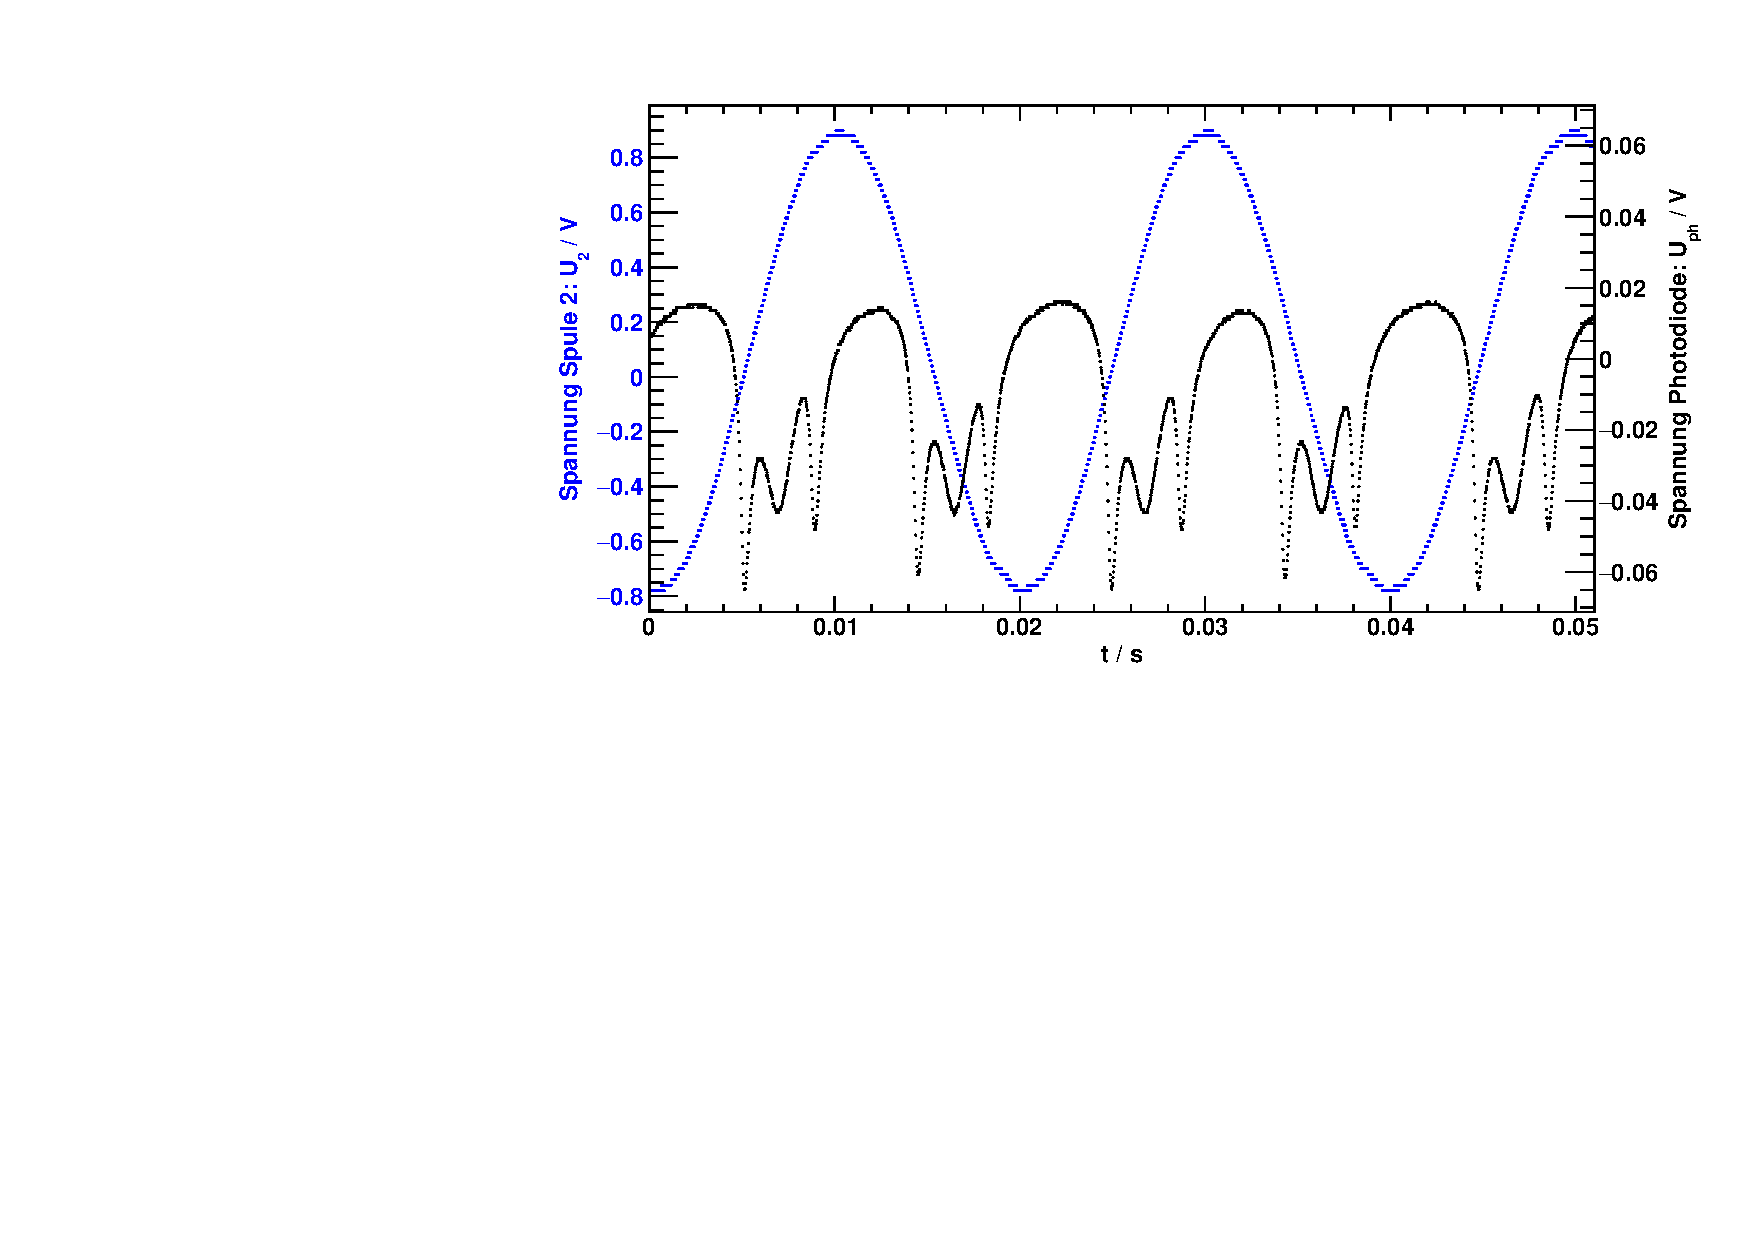
\includegraphics[width=\textwidth]{../img/part3/06.pdf}
  \caption{Starke Modulation des Magnetfelds in Strahlrichtung mit Spule~2 (schwarz).
   Im Photodiodensignal (rot) sind vier Doppelresonanz-Peaks sowie
   zwei Dehmelt-Peaks pro Modulationsperiode sichtbar.}
  \label{img:dehmeltrf}
\end{center}
\end{figure}

\begin{figure}[H]
\begin{center}
    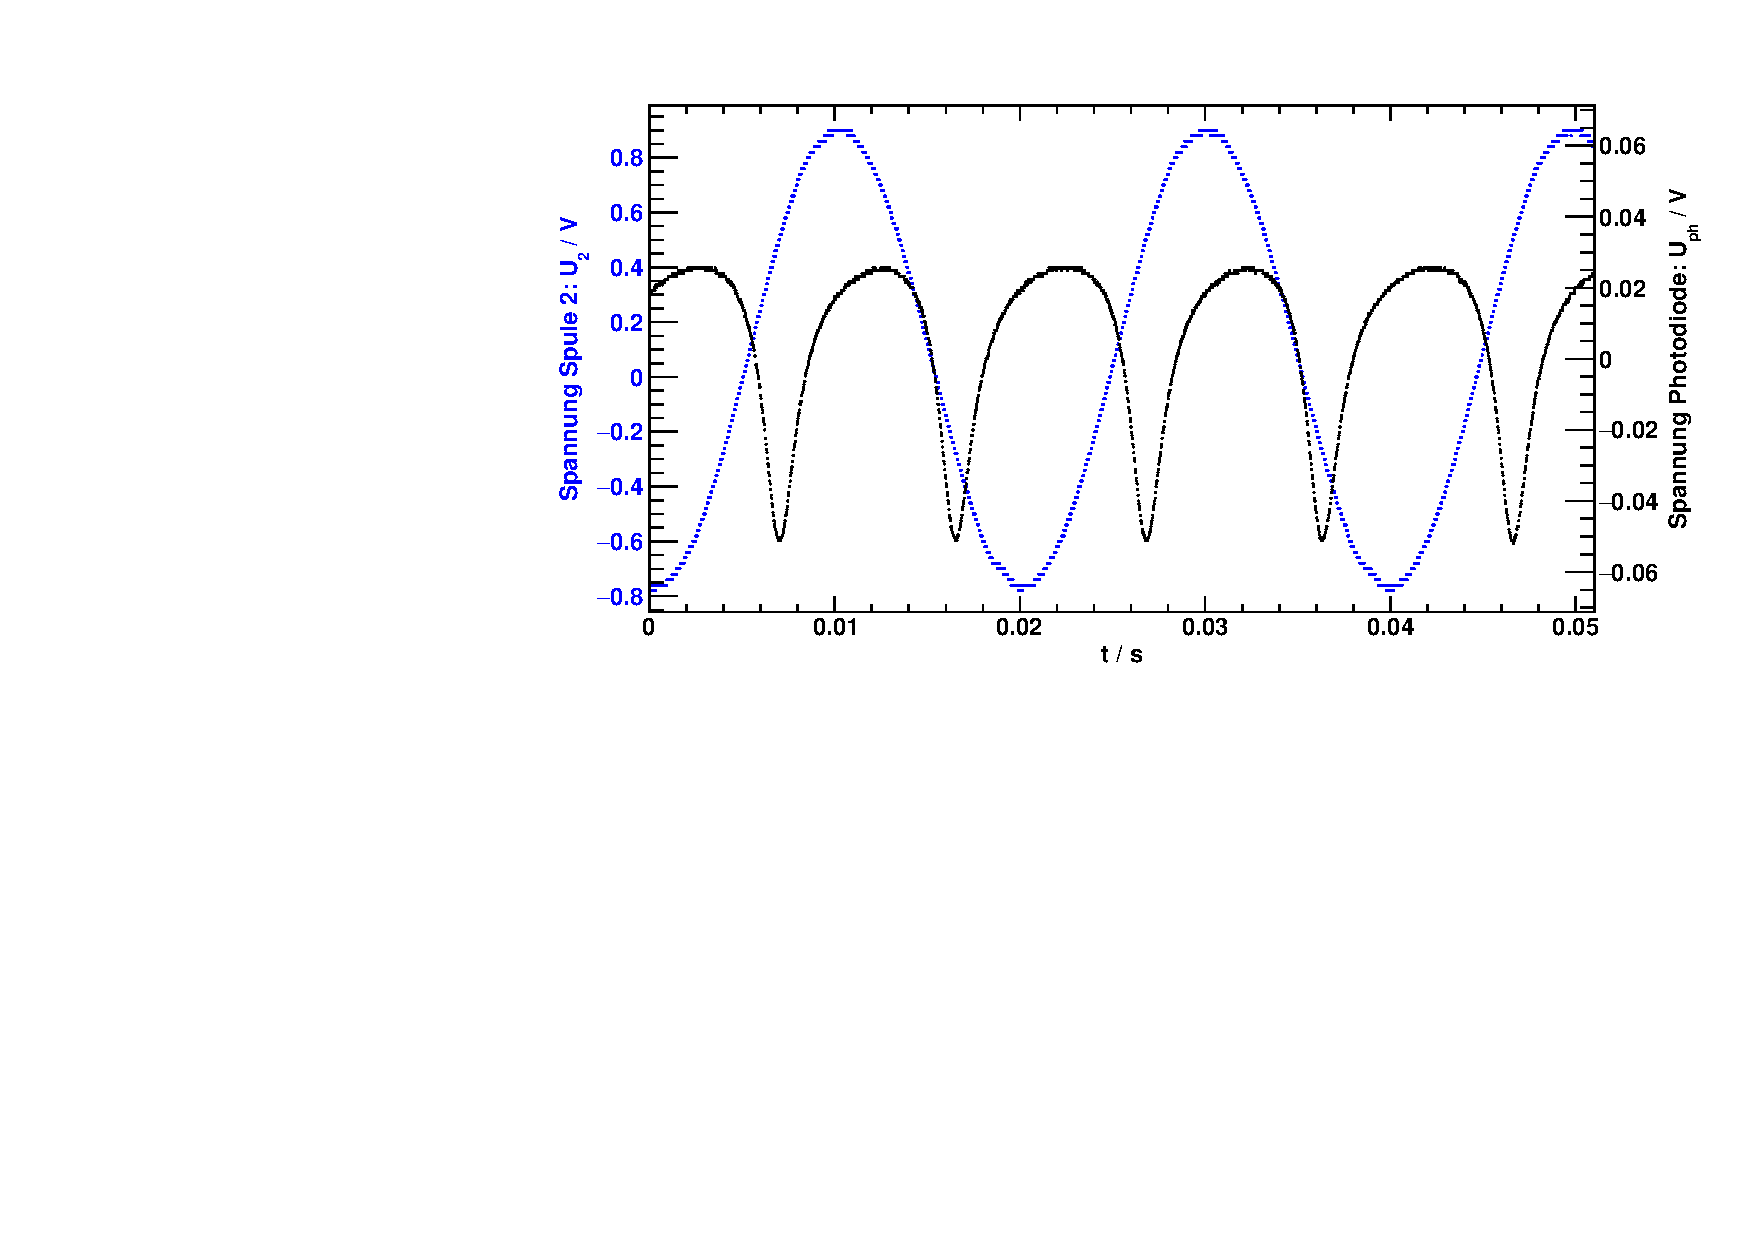
\includegraphics[width=\textwidth]{../img/part3/07.pdf}
    \caption{Gleiches Setup wie bei \autoref{img:dehmeltrf}, aber ohne RF-Signal.
    Die Dehmelt-Peaks sind weiterhin vorhanden.}
    \label{img:dehmelt}
\end{center}
\end{figure}

\begin{figure}[H]
\begin{center}
  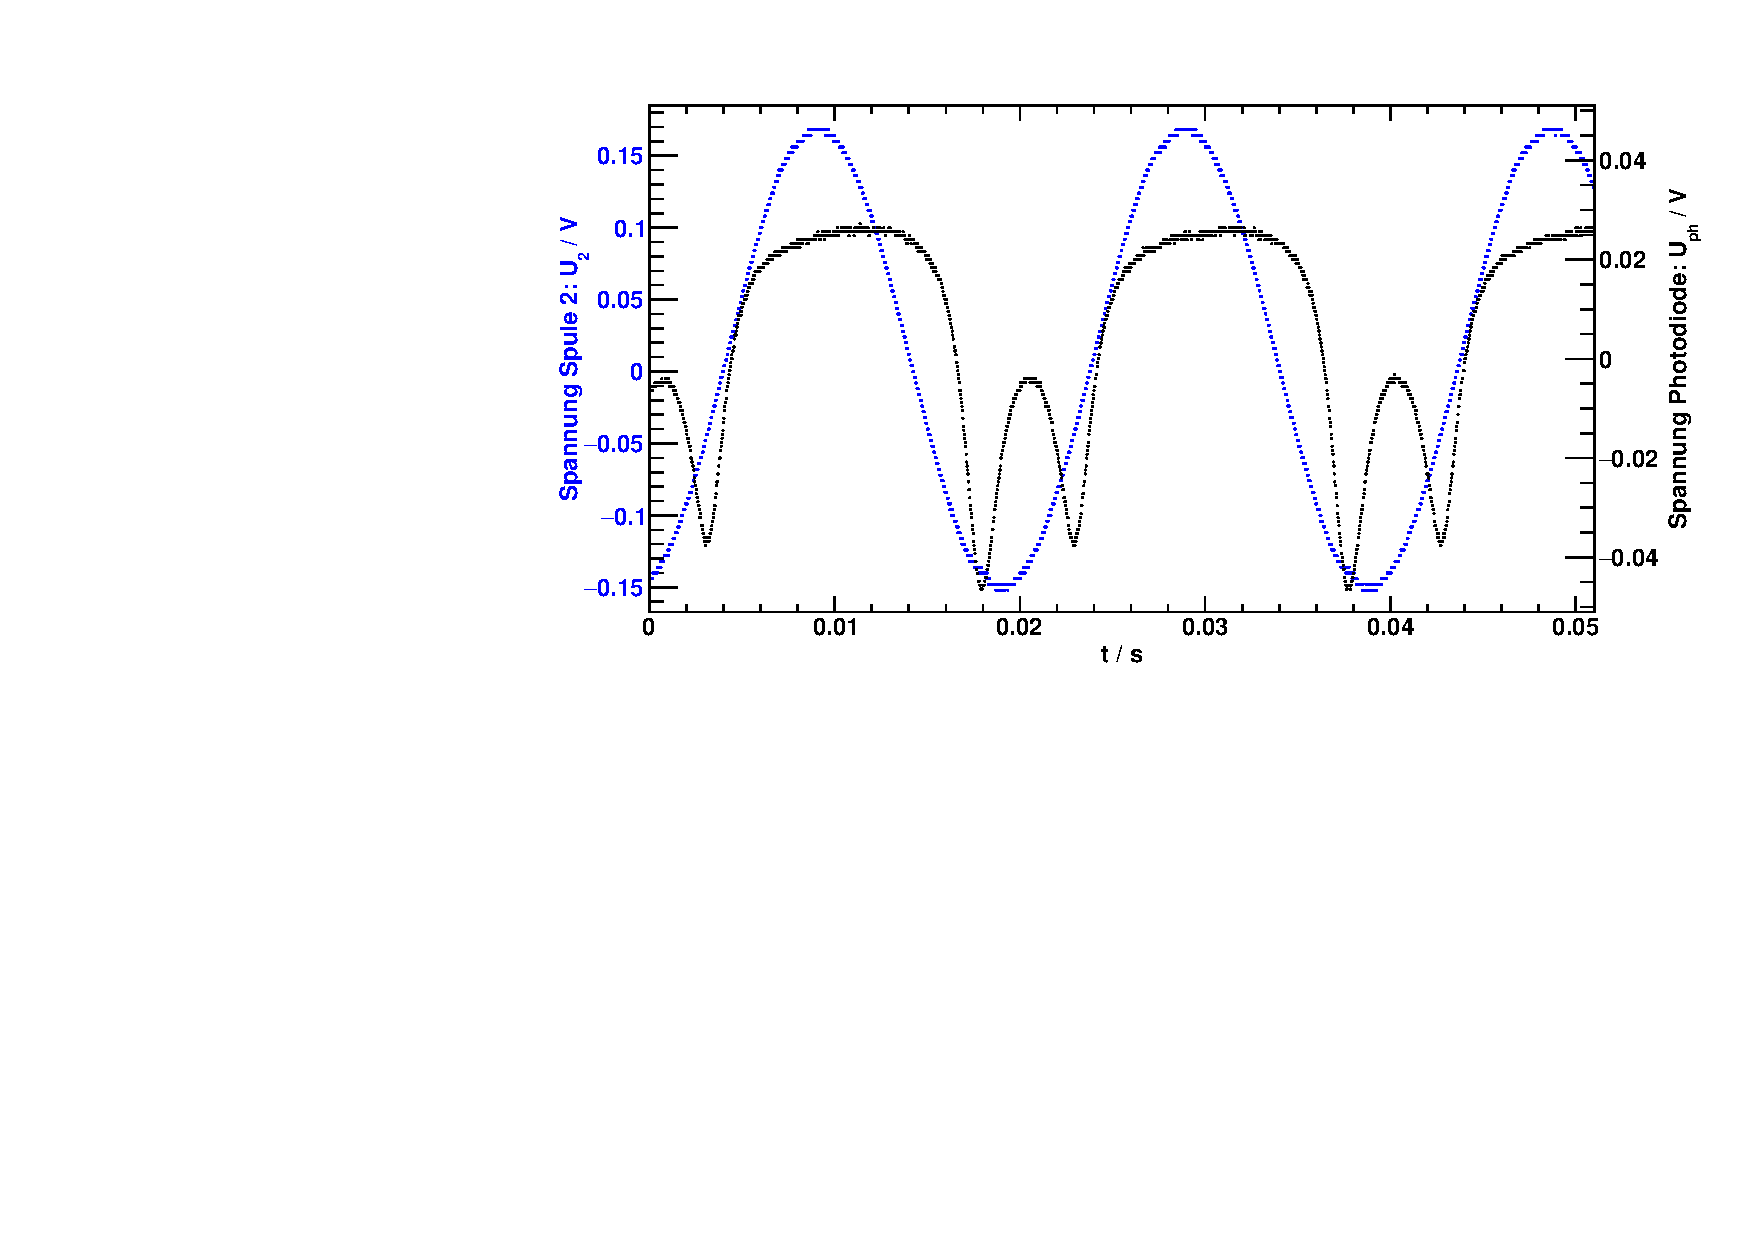
\includegraphics[width=\textwidth]{../img/part3/11.pdf}
  \caption{Doppelresonanz-Absorptionssignal bei kleiner Magnetfeldmodulation:
  Falsche Einstellung des Gleichstroms in Spule~1,
  die Absorptionen sind nicht äquidistant.}
  \label{img:rfwrong}
\end{center}
\end{figure}

\begin{figure}[H]
\begin{center}
  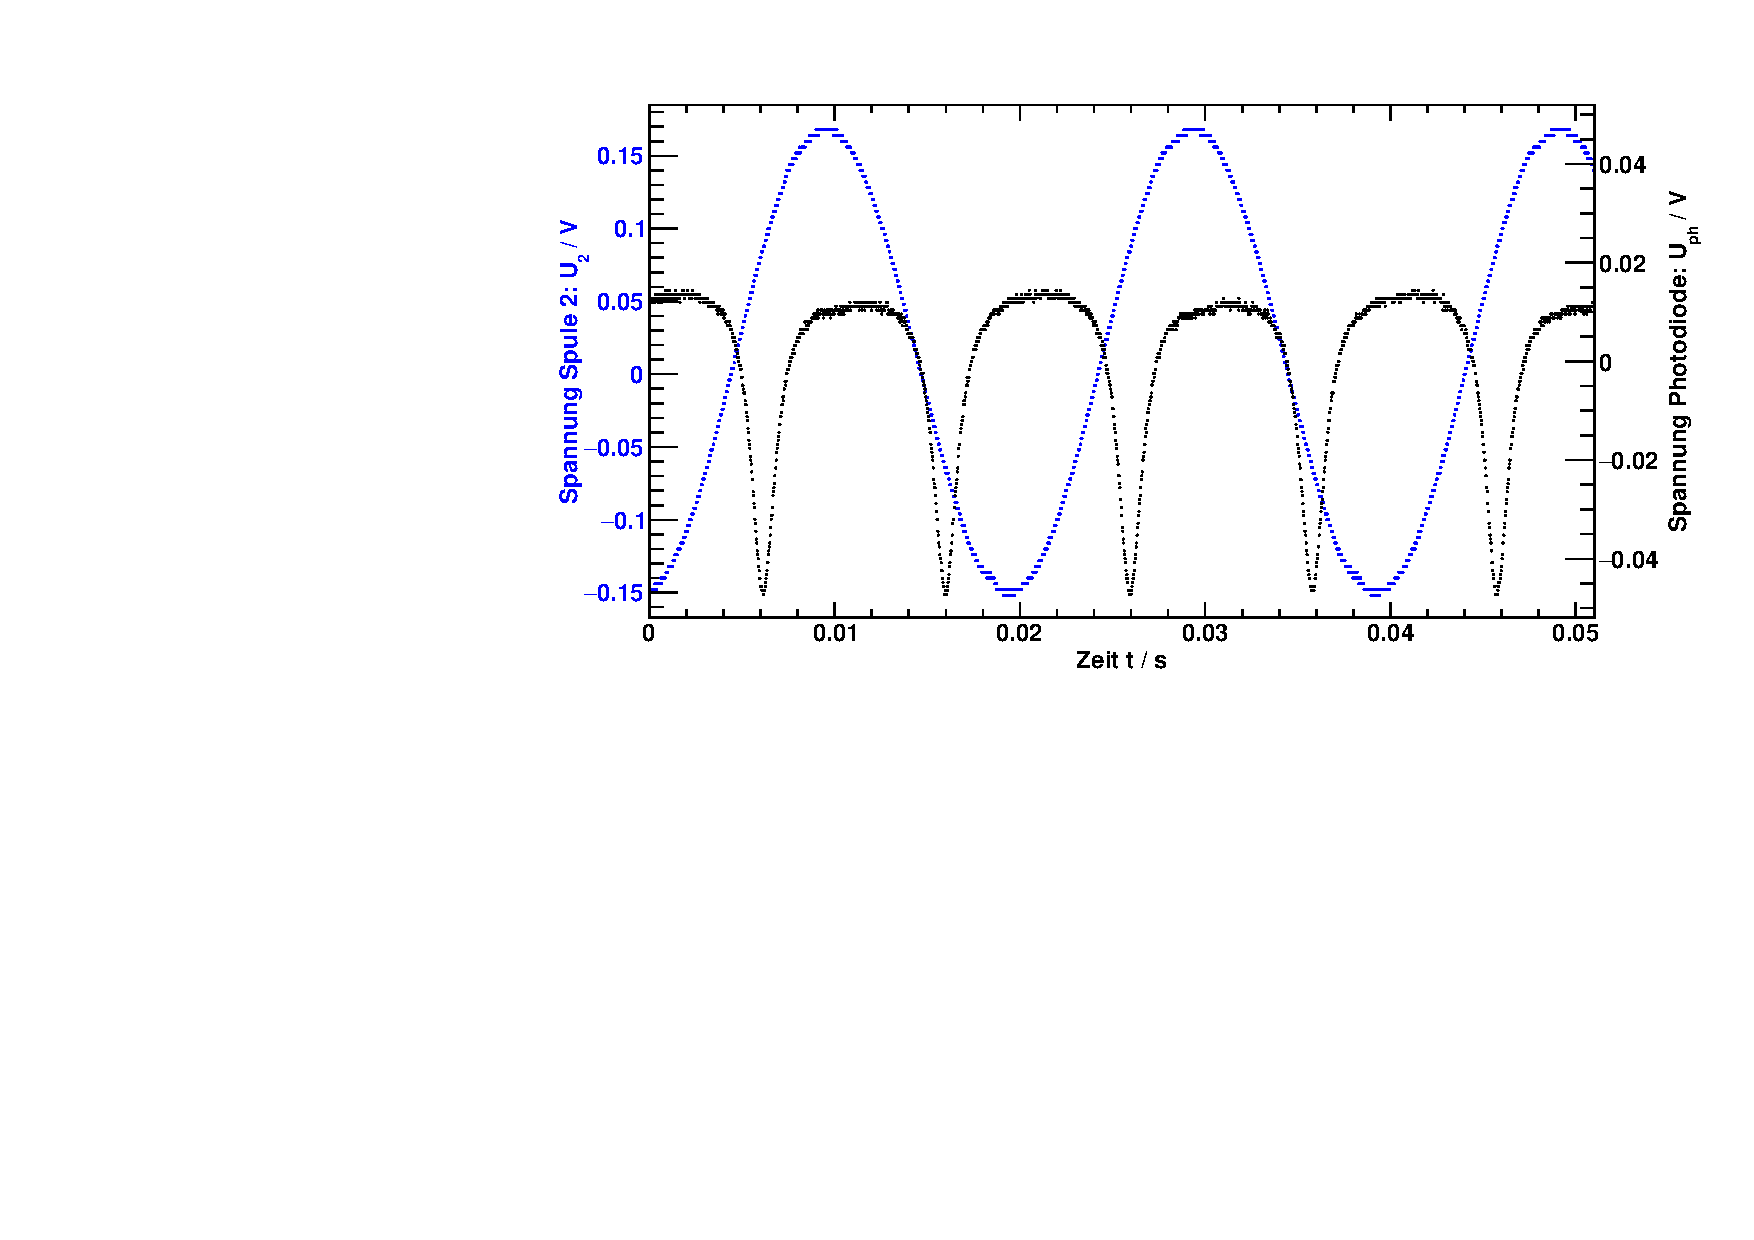
\includegraphics[width=\textwidth]{../img/part3/08.pdf}
  \caption{Doppelresonanz-Absorptionssignal bei kleiner Magnetfeldmodulation:
  Korrekte Einstellung des Gleichstroms in Spule~1,
  die Absorptionen sind daher äquidistant.}
  \label{img:rfcorrect}
\end{center}
\end{figure}

\subsection{Auswertung}
\subsubsection*{Berechnung des horizontalen und vertikalen Magnetfeldes und des Kernspins}
Die durch die Messung erhaltenen Ströme, welche durch Spule 1 ($I_1$ und bei Umpolung $I_1'$) fließen, sind in \autoref{tab:part3:data} 
aufgelistet. Der Strom $I_4$ von Spule beträgt in allen Fällen
\begin{equation}
    I_4 = (86 \pm 3)\,\text{mA}
\end{equation}
Die Fehler auf den Laserstrom $I_L$ und die Frequenz $\nu$ des RF-Senders sind $s_{I_L} = 0.1$\,mA und $s_\nu=0.1$\,kHz. 
\begin{table}[H]
\caption{Messdaten des Doppelresonanzexperiments.}
\begin{center}
\begin{tabular}{|c|c|c|c|c|c|}
  \hline
  $I_\text{L}$ / mA & $\nu$ / kHz & $I_1$ / mA & $s_{I_1}$ / mA & $I_1'$ / mA & $s_{I_1'}$ / mA \\ \hline
  62.9 & 493.98 & 117 & 2 & 148 & 2 \\ \hline
  62.9 & 899.41 & 228 & 4 & 260 & 4 \\ \hline
  63.2 & 493.77 & 104 & 2 & 74 & 2 \\ \hline
  63.2 & 899.67 & 148 & 2 & 179 & 2 \\ \hline
\end{tabular}
\end{center}
\label{tab:part3:data}
\end{table}

Zuerst wird der Strom in den Spulen in das resultierende Magnetfeld mit den Faktoren $c_n$ in \autoref{tab:inductorItoB} umgerechnet.
\begin{equation}
    B_n = c_n \cdot I, \qquad s_{B} = B_n \cdot \sqrt{ \left( \frac{s_I}{I} \right)^2 + \left( \frac{s_{c_n}}{c_n} \right)^2 }
\end{equation}
Nun können das horizontale und vertikale Magnetfeld, $B_\text{hor}$ und $B_\text{ver}$, sowie der Kernspin von Rubidium bestimmt werden.
\begin{itemize}
    \item Zur Bestimmung des horizontalen Magnetfeldes $B_\text{hor}$ wird die Hälfte des Mittelwerts von $B_1$ und $B_1'$ berechnet:
    \begin{equation}
        B_\text{hor} = \frac{1}{2} \abs{B_1 - B_1'}, \qquad s_{B_\text{hor}} = \frac{1}{2} \sqrt{s_{B_1}^2 + s_{B_1'}^2}
    \end{equation}
    \item Die Stärke des vertikalen Magnetfeldes $B_\text{ver}$ ergibt sich direkt aus der Stärke von Spule 4:
    \begin{equation}
        B_\text{ver} = B_4
    \end{equation}
    \item Um den Kernspin zu berechnen, muss von dem gemessenen Magnetfeld $B_1$ bzw. $B_1'$ das horizontale Erdmagnetfeld addiert oder - je nach
    Polung - subtrahiert werden. Bildet man aus diesen zwei Werten den Mittelwert, so kürzt sich das Erdmagnetfeld heraus und es ergibt sich
    folgende Formel:
    \begin{equation}
        B_I = \frac{B_1 + B_1'}{2}, \qquad s_{B_I} = \frac{1}{2} \sqrt{s_{B_1}^2 + s_{B_1'}^2}
    \end{equation}
    Mit diesem Wert und der Frequenz $\nu$ des RF-Senders kann nun mit \autoref{eq:nuclearspin} der Kernspin $I$ bestimmt werden.
    \begin{equation}
        I = \frac{\mu_B \cdot B_I}{h \cdot \nu} - \frac{1}{2}, \qquad s_I = \frac{\mu_B \cdot B_I}{h \cdot \nu} \sqrt{ \left( \frac{s_{B_I}}{B_I} \right)^2 + \left( \frac{s_\nu}{\nu} \right)^2}
    \end{equation}
\end{itemize}
\begin{table}[H]
\caption{Berechnete horizontale Komponenten des Erdmagnetfeldes und Kernspin von Rubidium für das Doppelresonanzexperiment bei verschiedenen Lasterströmen $I_\text{L}$ und RF-Sender Frequenzen $\nu$.}
\begin{center}
\begin{tabular}{|c|c|c|c|c|c|}
  \hline
  $I_\text{L}$ / mA & $\nu$ / kHz & $B_\text{hor}$ / \textmu T & $s_{B_\text{hor}}$ / \textmu T & $I$ & $s_I$ \\ \hline
  62.9 & 493.98 & 12.4 & 1.1 & 2.50 & 0.03 \\ \hline
  62.9 & 899.41 & 12.8 & 2.3 & 2.53 & 0.04 \\ \hline
  63.2 & 493.77 & 12.0 & 1.1 & 1.52 & 0.03 \\ \hline
  63.2 & 899.67 & 12.4 & 1.1 & 1.53 & 0.02 \\ \hline
\end{tabular}
\end{center}
\label{tab:part3:results}
\end{table}

\subsubsection*{Nennung der berechneten Werte und Vergleich mit Literatur- bzw. theoretischen Werten.}
In \autoref{tab:part3:results} sind die berechneten Werte des horizontale Erdmagnetfeldes für die verschiedenen Laserspannungen $I_L$ und 
RF-Sender Frequenzen $\nu$ zusammengestellt. 
\begin{itemize}
    \item Das vertikale Erdmagnetfeld ergibt sich zu
    \begin{equation}
        B_\text{ver} = (40.94 \pm 1.43)\,\text{\textmu T}\ \, ,
    \end{equation}
    was sich mit dem Literaturwert\footnote{Die Literaturwerte des horizontalen und vertikalen Erdmagnetfeldes, sowie die theoretischen Werte der
    Kernspins wurden \cite{manual} entnommen.} innerhalb von einem 2-\textsigma-Intervall deckt.
    \begin{equation}
        B_\text{ver}^{\text{Lit.}} = 42.9\,\text{\textmu T}
    \end{equation}
    \item Aus den Werten und Fehlern des horizontalen Magnetfeldes wird das gewichtete Mittel gebildet. Man erhält
    \begin{equation}
        \bar{B}_\text{hor} = (12.3 \pm 0.6)\,\text{\textmu T}\ \, .
    \end{equation}
    Dies stimmt nicht mit dem Literaturwert überein.
    \begin{equation}
        B_\text{hor}^{\text{Lit.}} = 20.9\,\text{\textmu T}
    \end{equation}
    Grund dafür ist TODO Grund \\ %TODO Grund Bhor
    \item Auch die beiden Werte des Kernspins für jedes Isotop werden gewichtet gemittelt:
    \begin{equation}
        I(\text{\rb{85}}) = 2.51 \pm 0.02, \qquad I(\text{\rb{87}}) = 1.53 \pm 0.16
    \end{equation}
    Der errechnete Wert des Kernspins für \rb{85} stimmt innerhalb der Fehlergrenzen mit dem theoretischen Wert überein, für \rb{87} liegen
    errechneter und theoretischer Wert innerhalb des 2-\textsigma-Intervalls.
    \begin{equation}
        I(\text{\rb{85}})^\text{theo.} = 2.5, \qquad I(\text{\rb{87}})^\text{theo.} = 1.5
    \end{equation}
\end{itemize}